\documentclass{article}

\usepackage{physics}
\usepackage{graphicx}
\usepackage{hyperref}

\usepackage{listings}
\usepackage{color}

\definecolor{red}{rgb}{1,0,0}
\definecolor{dkgreen}{rgb}{0,0.6,0}
\definecolor{gray}{rgb}{0.5,0.5,0.5}
\definecolor{mauve}{rgb}{0.58,0,0.82}

\hypersetup{
    colorlinks=true,
    linkcolor=blue,
    filecolor=magenta,      
    urlcolor=blue,
}

\lstset{
    frame=tb,
    language=Bash,
    aboveskip=3mm,
    belowskip=3mm,
    showstringspaces=false,
    columns=flexible,
    basicstyle={\small\ttfamily},
    numbers=none,
    numberstyle=\tiny\color{gray},
    keywordstyle=\color{blue},
    commentstyle=\color{dkgreen},
    stringstyle=\color{mauve},
    breaklines=true,
    breakatwhitespace=true,
    tabsize=3
}

\title{COVID-19 Data Analysis}

\author{Rishav Bhagat}

\graphicspath{{../res/imgs/}}

\begin{document}
    \maketitle
    \section{Dataset}
        I used the dataset that was collected and used by John Hopkins University for 
        \href{https://www.arcgis.com/apps/opsdashboard/index.html#/bda7594740fd40299423467b48e9ecf6}{this project}. 
        This dataset was collected from many international health organizations and all compiled into onto github repository. 
        It contains information on daily reports (including new cases, deaths, and recoveries), and global trends. 
        \newline \indent
        Here is the link to the datasets I used: 
        \newline\indent\indent \href{https://github.com/CSSEGISandData/COVID-19}{https://github.com/CSSEGISandData/COVID-19}
        \subsection{Downloading the Data}
            I created a batch script to download all this data using git, delete files that are not needed for my analysis, and move the files into more convienient locations.
            \begin{lstlisting}
                @echo off
                rmdir data /s /q
                git clone https://github.com/CSSEGISandData/COVID-19.git
                rename COVID-19 data
                cd data
                rmdir .git /s /q
                rmdir archived_data /s /q
                rmdir who_covid_19_situation_reports /s /q
                del README.md
                mv csse_covid_19_data/* .
                rmdir csse_covid_19_data /s /q
                cd ..
                git add data
                git commit -m "updated data from John Hopkins github repo"
                git push
            \end{lstlisting}
        \subsection{Initial Analysis}
            First, I plotted the global coronavirus data (cases vs days) in a similar fashion to the way it was plotting on the John Hopkins project. This is to reveal any obvious trends.
            \begin{center}
                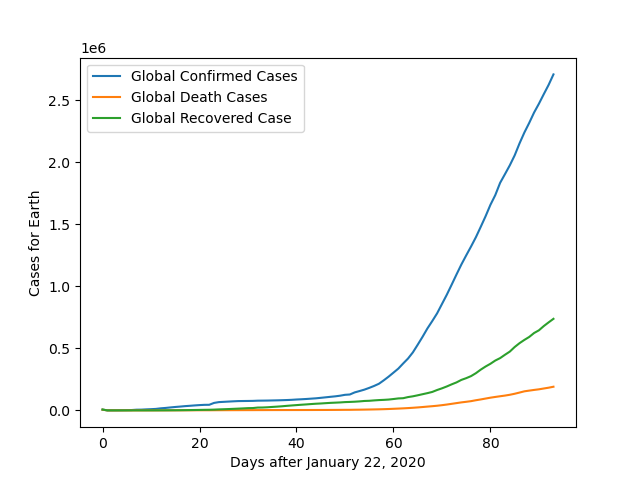
\includegraphics[width=10cm]{plots/global/cases.png}
            \end{center}

\end{document}